\subsection{Inhoudstypen}\label{inhoudstypen}
Inhoudstypen worden gebruikt voor het weergeven van verschillende typen inhoud. Per inhoudstype kunnen bijvoorbeeld verschillende velden gedefinieerd worden en de bijbehorende pagina's kunnen apart gestijled worden. Het gebruik van inhoudstypen cre{\"{e}}ert veel flexibiliteit.

\textbf{Relatie met E-suite:}  \emph{Drupal} zal automatisch content importeren uit de \emph{E-suite}. O.a. bekendmakingen, regelingen en producten worden automatisch ge{\"\i}mporteerd. 

In de volgende paragraaf zullen alle inhoudstypen nader beschreven worden.

\subsubsection{Agenda}\label{agenda}

\begin{enumerate}
\item Vul een titel in bij het veld 'Titel'.
\item Vul optioneel een introductie tekst in bij het veld 'Intro'.
\item Vul de hoofdtekst in bij het veld 'Body'.
\item Upload optioneel een afbeelding bij het veld 'Image'.
\item Specificeer optioneel een (eind)datum - kruis 'toon einddatum' aan om een einddatum te specificeren.
\item Specificeer optioneel een datum en tijd (bijvoorbeeld wanneer een evenement start) bij het veld 'Datum'.
\item Specificeer optioneel een locatie bij de velden onder 'Locatie'.
\item Voeg optioneel de content toe aan de kalender, dit doe je d.m.v. een datum te specificeren bij het veld 'Datum'.
\item Klik onderaan de pagina op de knop 'Opslaan' om de inhoud op te slaan.
\end{enumerate}

\subsubsection{Bekendmaking}\label{bekendmaking}

\emph{Bekendmakingen worden automatisch ge{\"\i}mporteerd.}

\begin{enumerate}
\item Vul een titel in bij het veld 'Titel'.
\item Selecteer het type bekendmaking.
\item Voeg optioneel de content toe aan de kalender, dit doe je d.m.v. een datum te specificeren bij het veld 'Datum'.
\item Vul de hoofdtekst in bij het veld 'Body'.
\item Specificeer optioneel een locatie bij de velden onder 'Locatie'.
\item Klik onderaan de pagina op de knop 'Opslaan' om de inhoud op te slaan.
\end{enumerate}

\subsubsection{Bericht}\label{bericht}

\begin{enumerate}
\item Vul een titel in bij het veld 'Titel'.
\item Vul de hoofdtekst in bij het veld 'Body'.
\item Klik onderaan de pagina op de knop 'Opslaan' om de inhoud op te slaan.
\end{enumerate}

\subsubsection{Bestand}\label{bestand}

\begin{enumerate}
\item Vul een titel in bij het veld 'Titel'.
\item Upload het gewenste bestand bij het veld 'Bestand'.
\item Klik onderaan de pagina op de knop 'Opslaan' om de inhoud op te slaan.
\end{enumerate}

\subsubsection{Bestemmingsplan}\label{bestemmingsplan}

\emph{Bestemmingsplannen worden automatisch ge{\"\i}mporteerd.}

\begin{enumerate}
\item Vul een titel in bij het veld 'Titel'.
\item Selecteer het type en de status van het bestemmingsplan bij de velden 'Type' en 'Status'
\item Voeg eventueel links toe naar documenten bij de velden 'Regels', 'Beleids document', 'Besluits document', 'Toelichting', 'Vastellings besluit', 'Bijlage' en/of 'Illustratie'. Vul een titel in en een url en klik op de knop 'Item toevoegen'. Herhaal deze stappen om meerdere links toe te voegen. 
\item Specificeer optioneel een locatie bij de velden onder 'Locatie'.
\item Klik onderaan de pagina op de knop 'Opslaan' om de inhoud op te slaan.
\end{enumerate}

\subsubsection{Blog}\label{blog}

\begin{enumerate}
\item Vul een titel in bij het veld 'Titel'
\item Upload optioneel een afbeelding bij het veld 'Image'
\item Vul optioneel een introductie tekst in bij het veld 'Intro'
\item Vul de hoofdtekst in bij het veld 'Body'.
\item Vul eventueel tags in, gescheiden met een spatie.
\item Klik onderaan de pagina op de knop 'Opslaan' om de inhoud op te slaan.
\end{enumerate}

\subsubsection{Editorial}\label{editorial}

\begin{enumerate}
\item Vul een titel in bij het veld 'Titel'
\item Vul de hoofdtekst in bij het veld 'Body'.
\item Klik onderaan de pagina op de knop 'Opslaan' om de inhoud op te slaan.
\end{enumerate}

\subsubsection{Eenvoudige pagina}\label{eenvoudigepagina}

\begin{enumerate}
\item Vul een titel in bij het veld 'Titel'.
\item Vul de hoofdtekst in bij het veld 'Body'.
\item Specificeer optioneel een locatie bij de velden onder 'Locatie'.
\item Klik onderaan de pagina op de knop 'Opslaan' om de inhoud op te slaan.
\end{enumerate}

\subsubsection{FAQ}\label{faq}

\begin{enumerate}
\item Vul een titel(vraag) in bij het veld 'Titel'.
\item Vul de hoofdtekst(antwoord) in bij het veld 'Body'.
\item Selecteer een FAQ Categorie bij het veld 'Categorie'.
\item Klik onderaan de pagina op de knop 'Opslaan' om de inhoud op te slaan.
\end{enumerate}

\subsubsection{Forumonderwerp}\label{forumonderwerp}

\begin{enumerate}
\item Vul een onderwerp in bij het veld 'Onderwerp'.
\item Selecteer een Forum Categorie bij het veld 'Forums'.
\item Vul de hoofdtekst in bij het veld 'Body'.
\item Klik onderaan de pagina op de knop 'Opslaan' om de inhoud op te slaan.
\end{enumerate}

\subsubsection{Foto}\label{foto}

\begin{enumerate}
\item Vul een titel in bij het veld 'Titel'.
\item Vul eventueel de hoofdtekst(uitgebreide foto omschrijving) in bij het veld 'Body'.
\item Upload een foto bij het veld 'Foto'.
\item Vul minstens 1 tag in bij het veld 'Tags', scheid meerdere tags met een spatie
\item Klik onderaan de pagina op de knop 'Opslaan' om de inhoud op te slaan.
\end{enumerate}

\subsubsection{Marktplaats}\label{marktplaats}

\begin{enumerate}
\item Vul een titel in bij het veld 'Titel'.
\item Vul eventueel een intro in bij het veld 'Intro'
\item Vul de hoofdtekst in bij het veld 'Body'.
\item Selecteer een categorie(aangeboden of gevraagd) bij het veld 'Categorie'.
\item Klik onderaan de pagina op de knop 'Opslaan' om de inhoud op te slaan.
\end{enumerate}

\subsubsection{Nieuws}\label{nieuws}

\begin{enumerate}
\item Vul een titel in bij het veld 'Titel'.
\item Vul eventueel een intro in bij het veld 'Intro'
\item Vul de hoofdtekst in bij het veld 'Body'.
\item Upload optioneel een afbeelding bij het veld 'Image'.
\item Vul eventueel tags in, gescheiden met een spatie.
\item Specificeer optioneel een locatie bij de velden onder 'Locatie'.
\item Klik onderaan de pagina op de knop 'Opslaan' om de inhoud op te slaan.
\end{enumerate}

\subsubsection{Onderwerp}\label{onderwerp}

\begin{enumerate}
\item Vul een titel in bij het veld 'Titel'.
\item Vul de hoofdtekst in bij het veld 'Body'.
\item Klik onderaan de pagina op de knop 'Opslaan' om de inhoud op te slaan.
\end{enumerate}

\subsubsection{Peiling}\label{peiling}

\begin{enumerate}
\item Vul een vraag in bij het veld 'Vraag'.
\item Vul minstens twee mogelijke antwoorden in bij het veld 'Keuze', klik op de knop 'Meer keuzes' om meerdere keuzes te specificeren.
\item Bepaal bij het veld 'Peilingsstatus' of de Peiling 'gesloten' of 'actief' is.
\item Selecteer hoe lang de Peiling moet duren bij het veld 'Peilingsduur'.
\item Specificeer optioneel een locatie bij de velden onder 'Locatie'.
\item Klik onderaan de pagina op de knop 'Opslaan' om de inhoud op te slaan.
\end{enumerate}

\subsubsection{Persoon}\label{persoon}

\begin{enumerate}
\item Vul een titel in bij het veld 'Titel'.
\item Upload optioneel een afbeelding bij het veld 'Image'.
\item Selecteer minstens 1 categorie bij het veld 'Category'.
\item Vul de hoofdtekst in bij het veld 'Body'.
\item Klik onderaan de pagina op de knop 'Opslaan' om de inhoud op te slaan.
\end{enumerate}

\subsubsection{Product}\label{product}

\emph{Producten worden automatisch ge{\"\i}mporteerd.}

\begin{enumerate}
\item Vul een titel in bij het veld 'Titel'.
\item Vul een tekst in bij het veld 'Aanvraag', 'Beschrijving', 'Contact', 'Bezwaar', 'Kosten', 'Bijzonderheden' en 'Termijn'
\item Specificeer optioneel een locatie bij de velden onder 'Locatie'.
\item Maak 'Tabbed content' aan bij het veld 'Tabcontent'. Om meerdere tabs toe te voegen klik je op de knop 'Item toevoegen' onder het veld 'Tabcontent'.
\item Klik onderaan de pagina op de knop 'Opslaan' om de inhoud op te slaan.
\end{enumerate}

\subsubsection{RSS}\label{rss}

\emph{RSS items worden automatisch ge{\"\i}mporteerd.}

\subsubsection{RSS Source}\label{rsssource}
Met een 'RSS Source' kun je een uit een bron RSS Feeds ophalen.

\begin{enumerate}
\item Vul een titel in bij het veld 'Titel'.
\item Vul een URL in bij het veld 'URL'. Let op: de feed zal niet werken als de URL foutief is ingevuld.
\item Vul eventueel een hoofdtekst in bij het veld 'Body'.
\item Klik onderaan de pagina op de knop 'Opslaan' om de inhoud op te slaan.
\end{enumerate}

\subsubsection{Regeling}\label{regeling}

\emph{Regelingen worden automatisch ge{\"\i}mporteerd.}

\subsubsection{Slide}\label{slide}

\begin{enumerate}
\item Vul een titel in bij het veld 'Titel'.
\item Vul eventueel een URL in bij het veld 'Link', de 'Slide' zal doorlinken naar de opgegeven URL.
\item Upload een afbeelding bij het veld 'Image'.
\item Vul eventueel een hoofdtekst in bij het veld 'Body'.
\item Klik onderaan de pagina op de knop 'Opslaan' om de inhoud op te slaan.
\end{enumerate}

\subsubsection{VAC}\label{vac}

\emph{VAC items worden automatisch ge{\"\i}mporteerd.}

\begin{enumerate}
\item Vul een titel in bij het veld 'Titel'.
\item Vul een antwoord in bij het veld 'Antwoord'.
\item Vul een toelichting in bij het veld 'Toelichting'.
\item Klik onderaan de pagina op de knop 'Opslaan' om de inhoud op te slaan.
\end{enumerate}

\subsubsection{Wiki}\label{wiki}
Het inhoudstype 'wiki' zal worden gebruikt voor het aanmaken van informatieve pagina's.

Om een wiki pagina aan te maken ga je naar: \emph{Inhoud toevoegen} $\rightarrow$ \emph{Wiki} , of ga direct naar \drupalpath{node/add/wiki}.

Vul een titel bij het veld 'Titel' en vul informatieve tekst in bij het veld 'Body'.

Voor het inhoudstype 'Wiki' is een speciale filter gebouwd, deze filter maakt het refereren naar andere wiki pagina's mogelijk. 

Het refereren naar een andere wiki pagina gaat als volgt: 

\begin{enumerate}
\item Kopieer de titel van de node waarnaar je wilt refereren, bijvoorbeeld 'wiki pagina'
\item In de body tekst van je huidige node kun je refereren naar de node 'wiki pagina'
\item Plaats de node waarnaar je wilt refereren tussen dubbele 'square brackets': [[wiki pagina]]
\item Bijvoorbeeld: dit is informatie, op de pagina [[wiki pagina]] kun je meer informatie vinden.
\end{enumerate}

\bigskip

\begin{center}
	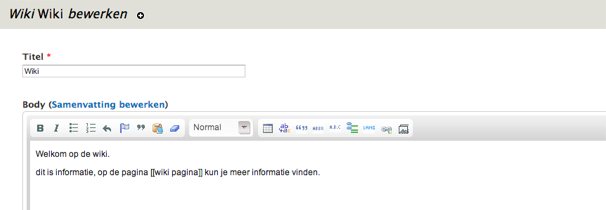
\includegraphics[width=\textwidth]{img/wiki.png}
\end{center}